% --------------------------------------------------------------------------- %
% --------------------------------------------------------------------------- %
\chapter{Results}
\label {ch:results}
% --------------------------------------------------------------------------- %
% --------------------------------------------------------------------------- %

In this section we provide the results of this search. 

\subsection{on-Z signal regions}

The results for SRA in the on-Z search are shown in this section.
The uncertainties in the tables and plots include the systematic uncertainties derived from the MC closure test.

\begin{table}[htb]
\scriptsize
\begin{center}
\caption{\label{tab:results_bveto_SRA} 
Results are shown for the b-veto, SRA.
Systematic uncertainties for each region are included in the total uncertainty. 
}
\begin{tabular}{l|c|c|c|c|c|c}
\hline
\hline
$\mathrm{E_{T}^{miss} [GeV]}$ &0 - 50 & 50 - 100 & 100 - 150 & 150 - 225 & 225 - 300 & $\geq$ 300 \\
\hline 
Z+jets&  1306.1 $\pm$ 62.3 &  307.1 $\pm$ 24.4 &  23.5 $\pm$ 4.4 &  4.3 $\pm$ 0.6 &  1.4 $\pm$ 0.4 &  1.0 $\pm$ 0.5 \\ 
FS bkg&  5.3$^{+ 3.6}_{- 2.3}$ &  9.5$^{+ 4.3}_{- 3.1}$ &  3.2$^{+ 3.1}_{- 1.7}$ &  3.2$^{+ 3.1}_{- 1.7}$ &  1.1$^{+ 2.4}_{- 0.9}$ &  0.0$^{+ 1.2}_{- 0.0}$ \\ 
Other SM&  1.6 $\pm$ 0.8 &  2.2 $\pm$ 1.0 &  1.5 $\pm$ 0.7 &  1.2 $\pm$ 0.6 &  0.8 $\pm$ 0.4 &  0.9 $\pm$ 0.5 \\ 
\hline 
total BG&  1313.0$^{+ 62.4}_{- 62.3}$ &  318.8$^{+ 24.8}_{- 24.6}$ &  28.2$^{+ 5.4}_{- 4.8}$ &  8.7$^{+ 3.2}_{- 1.9}$ &  3.3$^{+ 2.5}_{- 1.0}$ &  1.9$^{+ 1.4}_{- 0.7}$ \\ 
\hline 
Data&  1313 &  324 &  28 &  6 &  5 &  6 \\ 
\hline
\hline
\end{tabular}
\end{center}
\end{table}


\begin{table}[htb]
\scriptsize
\begin{center}
\caption{\label{tab:results_withb_SRA} 
Results are shown for the region with nbtags $\geq$ 1 in SRA.
Systematic uncertainties for each region are included in the total uncertainty. 
}
\begin{tabular}{l|c|c|c|c|c|c}
\hline
\hline
$\mathrm{E_{T}^{miss} [GeV]}$ &0 - 50 & 50 - 100 & 100 - 150 & 150 - 225 & 225 - 300 & $\geq$ 300 \\
\hline 
Z+jets&  180.7 $\pm$ 23.7 &  59.2 $\pm$ 16.7 &  4.4 $\pm$ 0.9 &  1.4 $\pm$ 0.4 &  0.7 $\pm$ 0.4 &  0.3 $\pm$ 0.2 \\ 
FS bkg&  5.3$^{+ 3.6}_{- 2.3}$ &  12.6$^{+ 4.8}_{- 3.6}$ &  9.5$^{+ 4.3}_{- 3.1}$ &  4.2$^{+ 3.3}_{- 2.0}$ &  4.2$^{+ 3.3}_{- 2.0}$ &  1.1$^{+ 2.4}_{- 0.9}$ \\ 
Other SM&  0.2 $\pm$ 0.1 &  0.2 $\pm$ 0.1 &  0.3 $\pm$ 0.1 &  0.2 $\pm$ 0.1 &  0.1 $\pm$ 0.0 &  0.2 $\pm$ 0.1 \\ 
\hline 
total BG&  186.0$^{+ 23.9}_{- 23.8}$ &  72.0$^{+ 17.4}_{- 17.1}$ &  14.2$^{+ 4.4}_{- 3.3}$ &  5.8$^{+ 3.4}_{- 2.1}$ &  5.0$^{+ 3.3}_{- 2.0}$ &  1.6$^{+ 2.4}_{- 0.9}$ \\ 
\hline 
Data&  186 &  67 &  21 &  6 &  1 &  3 \\ 
\hline
\hline
\end{tabular}
\end{center}
\end{table}

\begin{figure}[!ht]
\begin{center}
\begin{tabular}{cc}
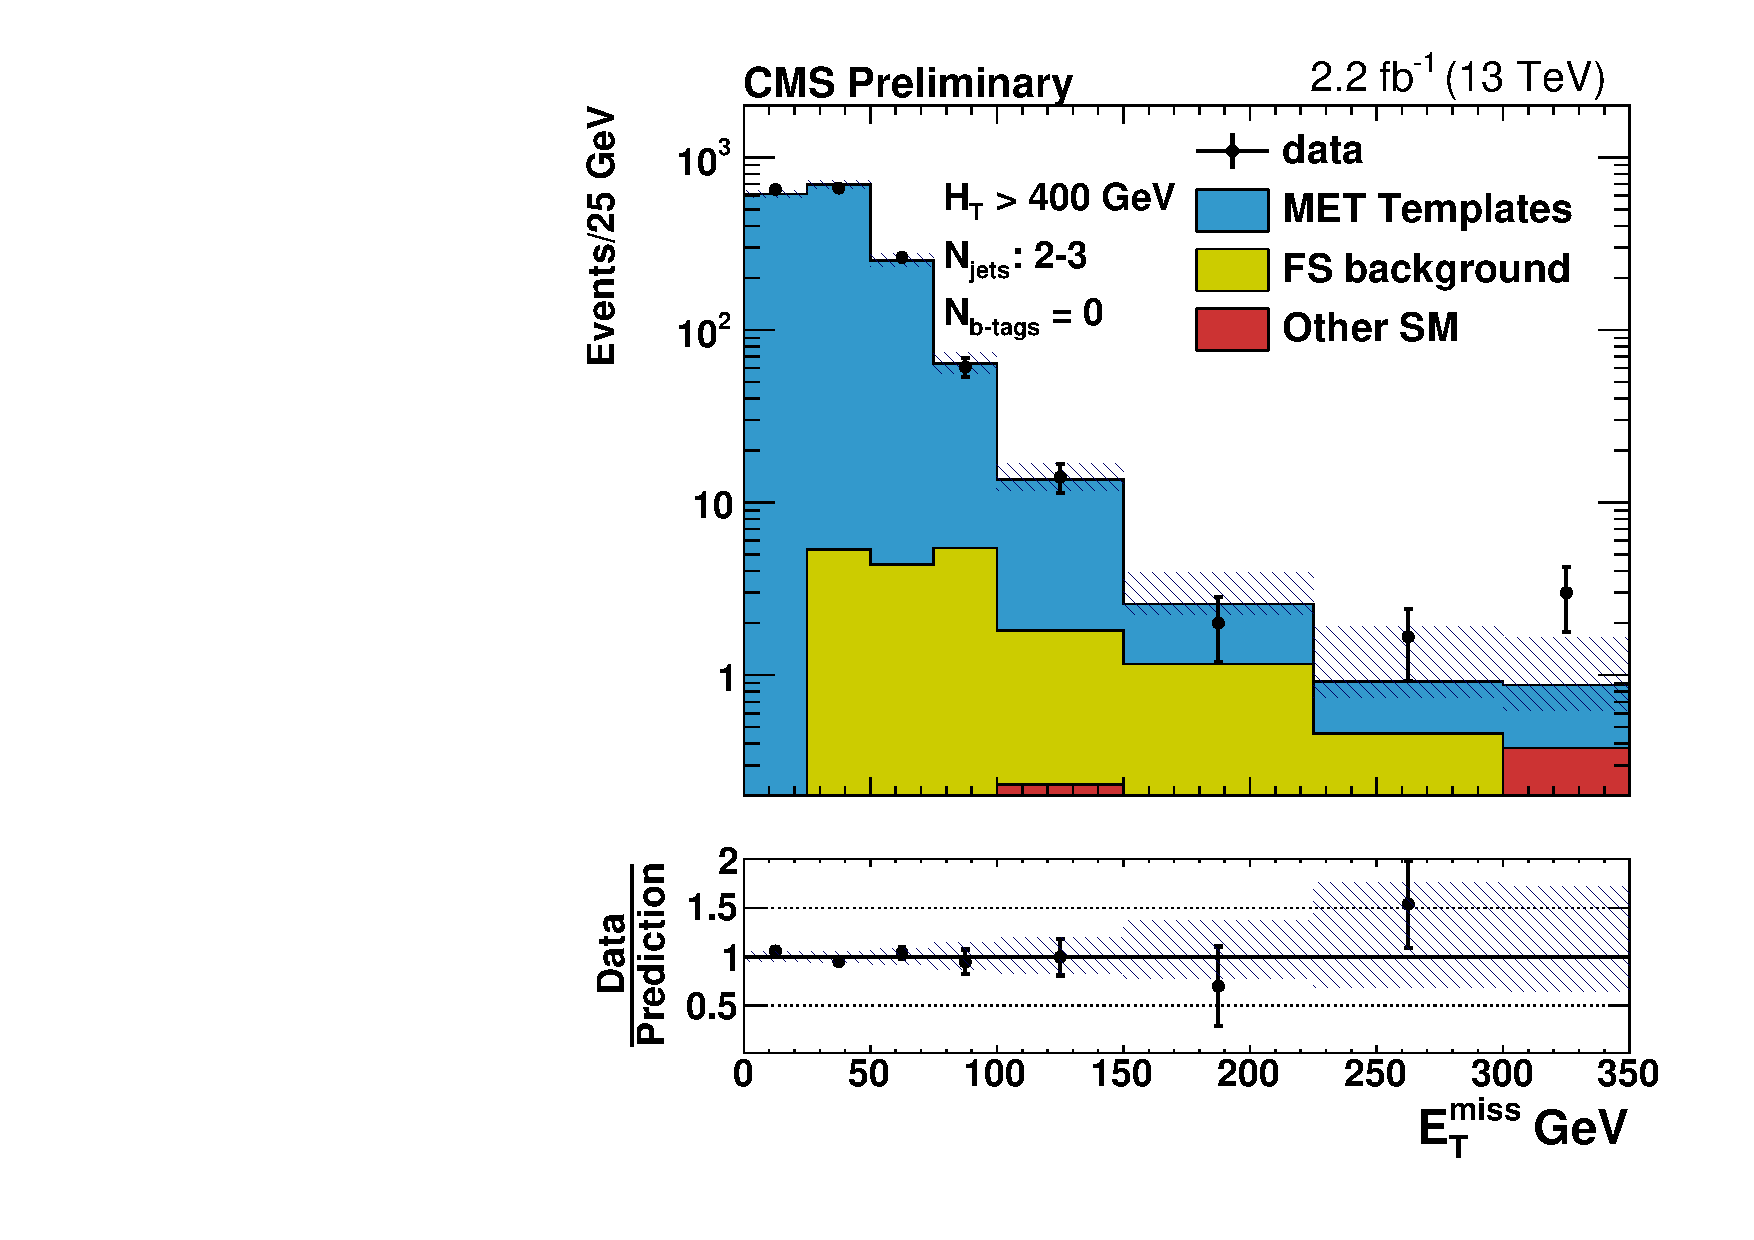
\includegraphics[width=0.4\textwidth]{results/figs/h_met_rawgt1jet_ll_signalregion_rawMET_loosephoton_bveto_SRA_fsbkg_passtrig.pdf} &
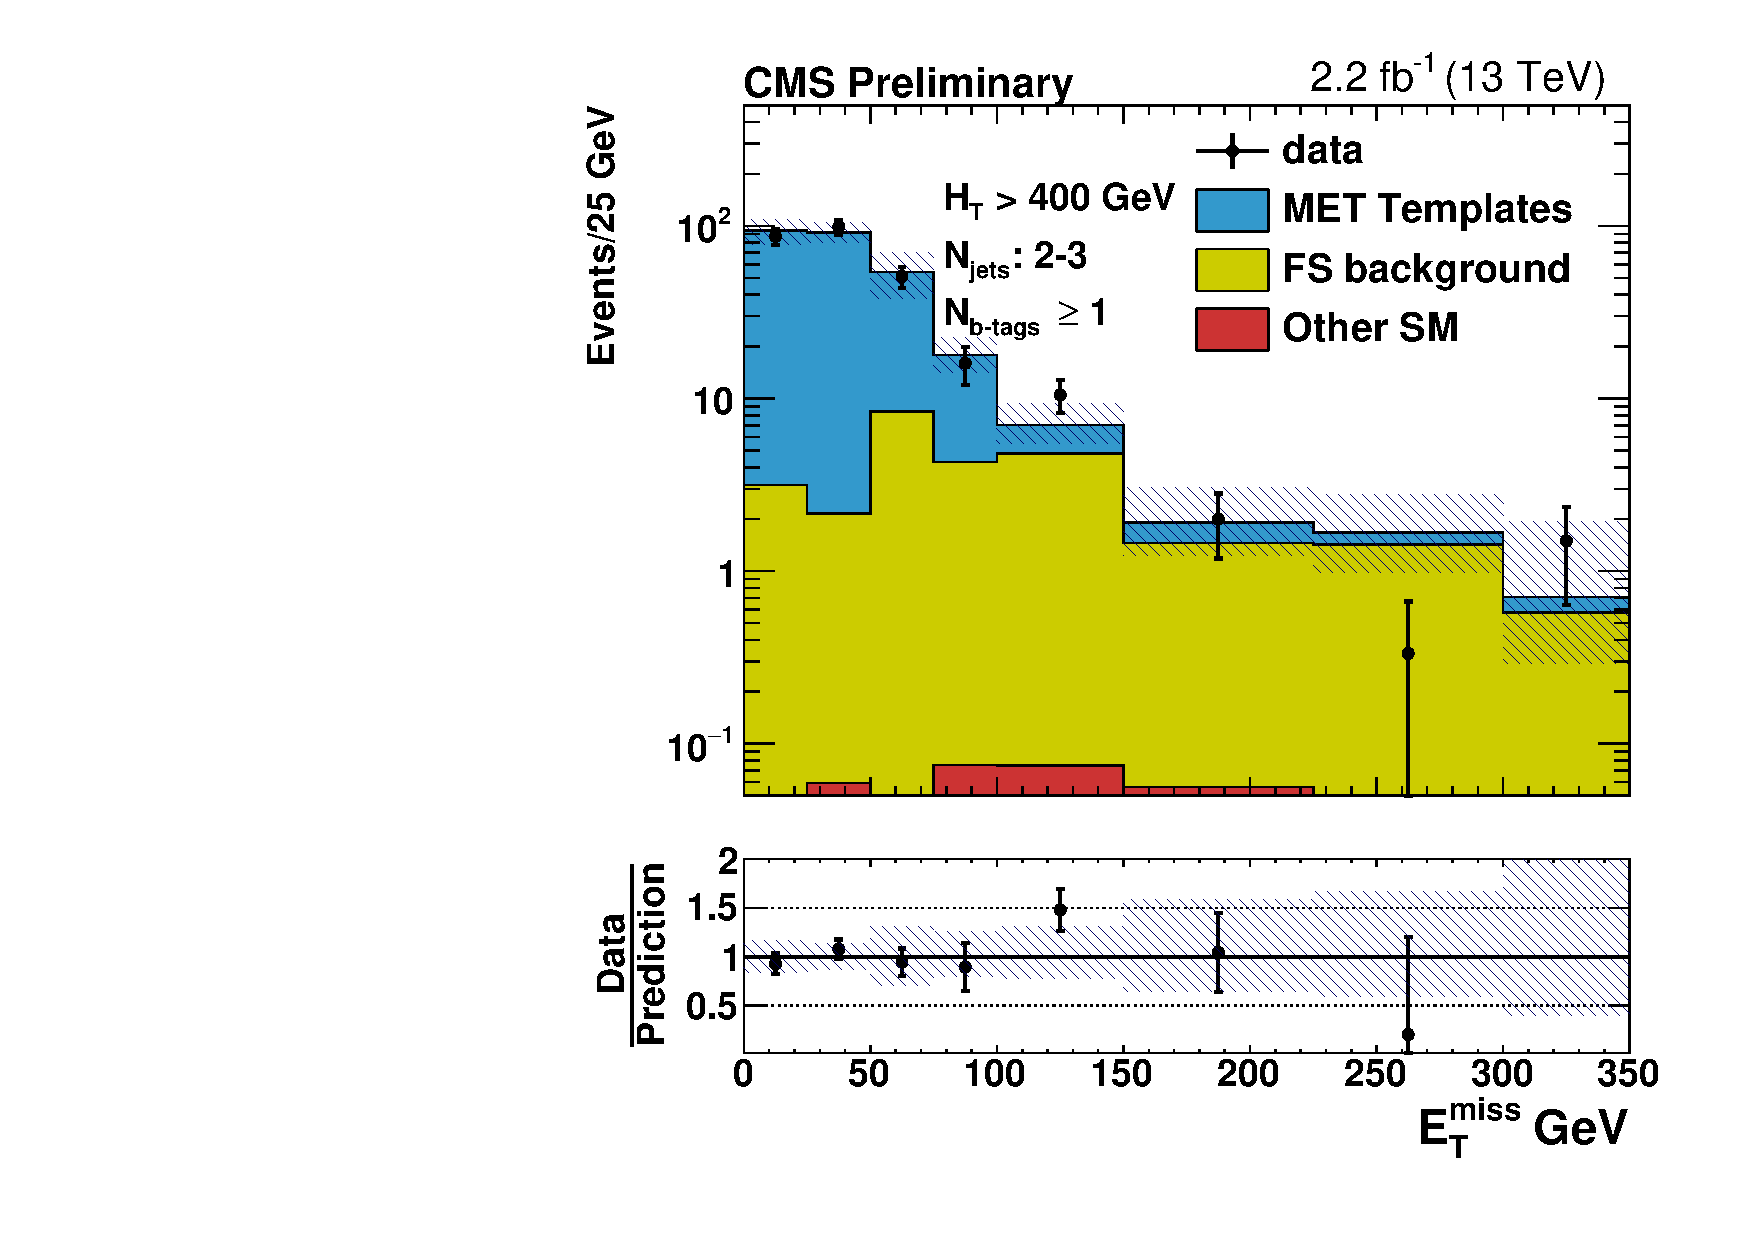
\includegraphics[width=0.4\textwidth]{results/figs/h_met_rawgt1jet_ll_signalregion_rawMET_loosephoton_withb_SRA_fsbkg_passtrig.pdf} \\
\end{tabular}
\caption{The \MET\ distribution is shown for data vs. the data-driven predictions in SRA.
The left plot shows the prediction when requiring N$\mathrm{_{b-jets}} =$ 0, and the right plot shows the prediction when requiring N$\mathrm{_{b-jets}} \geq$ 1.
See Tables~\ref{tab:results_bveto_SRA}~and~\ref{tab:results_withb_SRA}~for yields.
\label{fig:results_SRA}
}
\end{center}
\end{figure}

\clearpage


The results for SRB in the on-Z search are shown in this section.
The uncertainties in the tables and plots include the systematic uncertainties derived from the MC closure test.

\begin{table}[htb]
\scriptsize
\begin{center}
\caption{\label{tab:results_bveto_SRB} 
Results are shown for the b-veto, SRB.
Systematic uncertainties for each region are included in the total uncertainty. 
}
\begin{tabular}{l|c|c|c|c|c|c}
\hline
\hline
$\mathrm{E_{T}^{miss} [GeV]}$ &0 - 50 & 50 - 100 & 100 - 150 & 150 - 225 & 225 - 300 & $\geq$ 300 \\
\hline 
Z+jets&  1869.2 $\pm$ 68.0    &  276.9 $\pm$     16.2 &   9.6 $\pm$     0.9 &  3.2 $\pm$      0.6 &  0.4 $\pm$ 0.1 &  0.1 $\pm$ 0.1 \\ 
FS bkg&     9.5$^{+ 4.3}_{- 3.1}$ &   21.0$^{+ 5.9}_{- 4.7}$ &  12.6$^{+ 4.8}_{- 3.6}$ &  4.2$^{+ 3.3}_{- 2.0}$ &  0.0$^{+ 1.2}_{- 0.0}$ &  1.1$^{+ 2.4}_{- 0.9}$ \\ 
Other SM&   1.3 $\pm$ 0.6     &    1.9 $\pm$      0.8 &   0.9 $\pm$     0.4 &  0.8 $\pm$      0.3 &  0.4 $\pm$ 0.2 &  0.3 $\pm$ 0.1 \\ 
\hline 
total BG&  1880.0$^{+ 68.2}_{- 68.1}$ &  299.8$^{+ 17.3}_{- 16.9}$ &  23.1$^{+ 4.9}_{- 3.7}$ &  8.2$^{+ 3.4}_{- 2.1}$ &  0.8$^{+ 1.2}_{- 0.2}$ &  1.5$^{+ 2.4}_{- 0.9}$ \\ 
\hline 
Data&  1880 &  271 &  20 &  10 &  2 &  0 \\ 
\hline
\hline
\end{tabular}
\end{center}
\end{table}


\begin{table}[htb]
\scriptsize
\begin{center}
\caption{\label{tab:results_withb_SRB} 
Results are shown for the region with nbtags $\geq$ 1 in SRB.
Systematic uncertainties for each region are included in the total uncertainty. 
}
\begin{tabular}{l|c|c|c|c|c|c}
\hline
\hline
$\mathrm{E_{T}^{miss} [GeV]}$ &0 - 50 & 50 - 100 & 100 - 150 & 150 - 225 & 225 - 300 & $\geq$ 300 \\
\hline 
Z+jets&  410.4 $\pm$ 34.8 &  72.5 $\pm$ 8.0 &  4.9 $\pm$ 0.9 &  1.5 $\pm$ 0.3 &  0.4 $\pm$ 0.3 &  0.3 $\pm$ 0.2 \\ 
FS bkg&  49.4$^{+ 8.5}_{- 7.4}$ &  68.3$^{+ 9.9}_{- 8.8}$ &  38.9$^{+ 7.6}_{- 6.5}$ &  14.7$^{+ 5.1}_{- 3.9}$ &  0.0$^{+ 1.2}_{- 0.0}$ &  1.1$^{+ 2.4}_{- 0.9}$ \\ 
Other SM&  1.2 $\pm$ 0.5 &  1.5 $\pm$ 0.7 &  0.8 $\pm$ 0.4 &  0.5 $\pm$ 0.2 &  0.2 $\pm$ 0.1 &  0.1 $\pm$ 0.0 \\ 
\hline 
total BG&  461.0$^{+ 35.8}_{- 35.5}$ &  142.2$^{+ 12.8}_{- 12.0}$ &  44.6$^{+ 7.7}_{- 6.6}$ &  16.7$^{+ 5.1}_{- 3.9}$ &  0.6$^{+ 1.2}_{- 0.3}$ &  1.4$^{+ 2.4}_{- 0.9}$ \\ 
\hline 
Data&  461 &  149 &  43 &  22 &  3 &  3 \\ 
\hline
\hline
\end{tabular}
\end{center}
\end{table}

\begin{figure}[!ht]
\begin{center}
\begin{tabular}{cc}
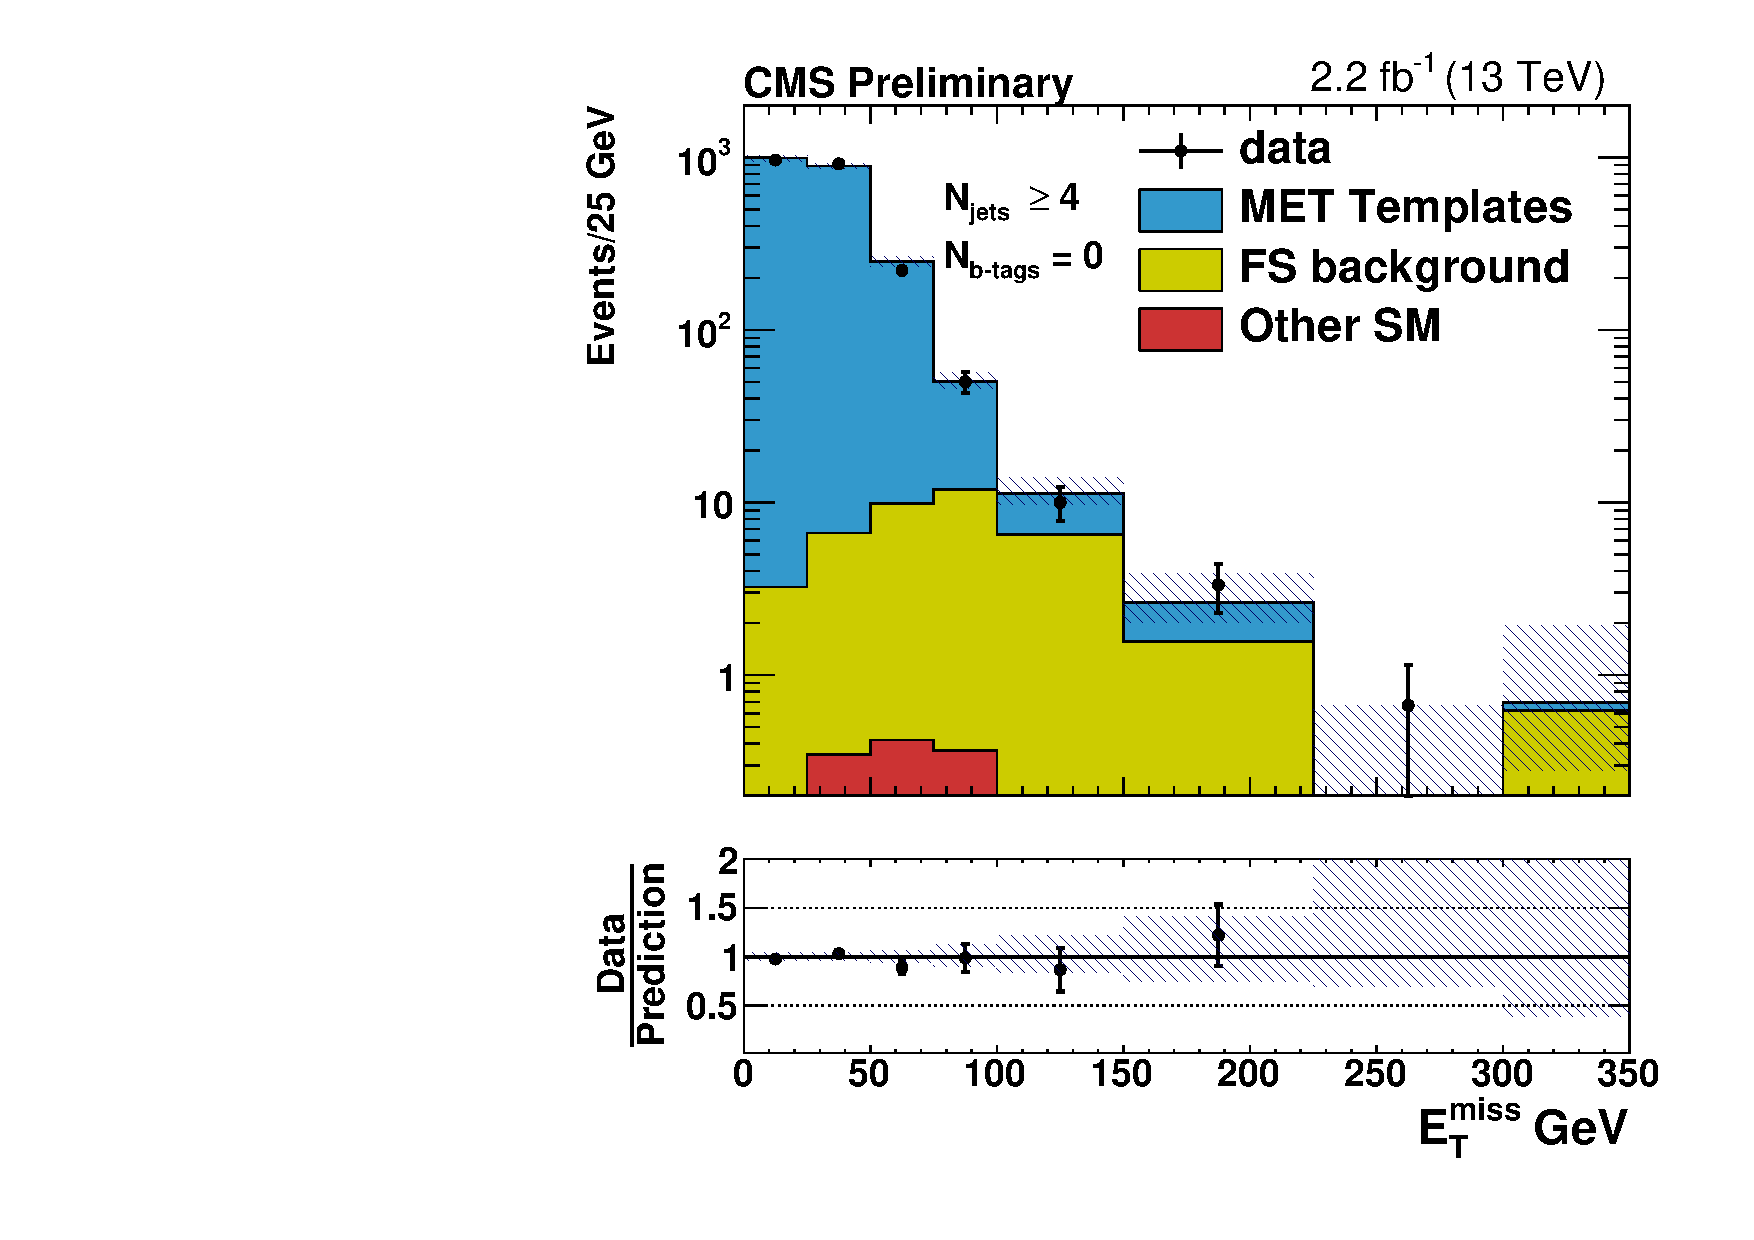
\includegraphics[width=0.4\textwidth]{results/figs/h_met_rawgt1jet_ll_signalregion_rawMET_loosephoton_bveto_SRB_fsbkg_passtrig.pdf} &
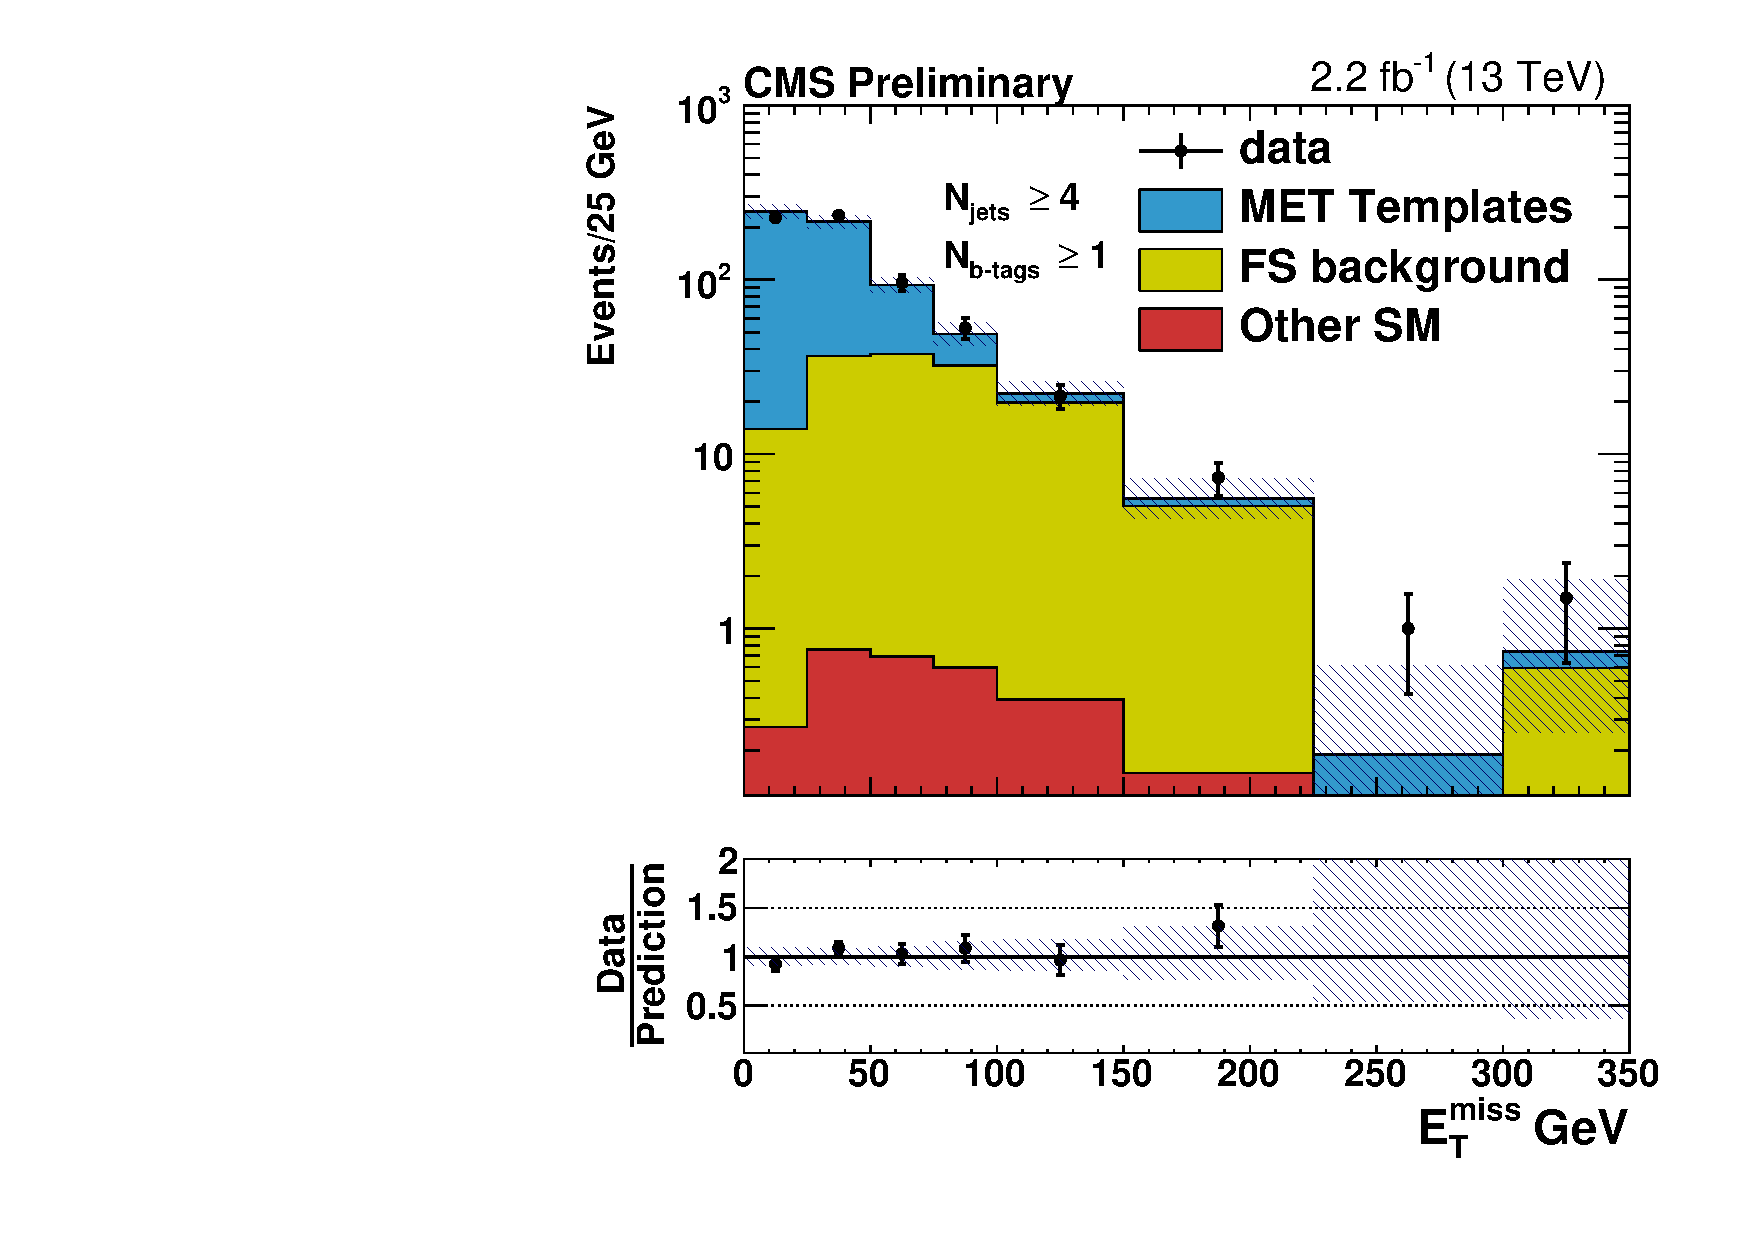
\includegraphics[width=0.4\textwidth]{results/figs/h_met_rawgt1jet_ll_signalregion_rawMET_loosephoton_withb_SRB_fsbkg_passtrig.pdf} \\
\end{tabular}
\caption{The \MET\ distribution is shown for data vs. the data-driven predictions in SRB.
The left plot shows the prediction when requiring N$\mathrm{_{b-jets}} =$ 0, and the right plot shows the prediction when requiring N$\mathrm{_{b-jets}} \geq$ 1.
See Tables~\ref{tab:results_bveto_SRB}~and~\ref{tab:results_withb_SRB}~for yields.
\label{fig:results_SRB}
}
\end{center}
\end{figure}

\clearpage


\subsection{ATLAS-like signal regions}

The results for the ATLAS-like signal region in the on-Z search are shown in this section.
The signal regions defined as \MET\ $\geq$ 225 \gev.
The uncertainties in the tables and plots include the systematic uncertainties derived from the MC closure test.

\begin{table}[htb]
\scriptsize
\begin{center}
\caption{\label{tab:results_SR_ATLAS} 
Results are shown for the ATLAS signal region.
Systematic uncertainties for each region are included in the total uncertainty. 
}
\begin{tabular}{l|c|c|c|c|c}
\hline
\hline
$\mathrm{E_{T}^{miss} [GeV]}$ &0 - 50 & 50 - 100 & 100 - 150 & 150 - 225 & $\geq$ 225 \\
\hline 
Z+jets  &  1535.3 $\pm$    64.7 &  376.1 $\pm$     18.8 &  33.4 $\pm$ 5.47     &  7.6 $\pm$      1.1 &  3.7 $\pm$     0.7 \\ 
FS bkg  &    20.0$^{+ 5.8}_{- 4.6}$ &  21.0 $^{+ 5.9}_{- 4.7}$ &  13.7 $^{+ 5.0}_{- 3.8}$ & 13.7$^{+ 5.0}_{- 3.8}$ &  6.3$^{+ 3.8}_{- 2.5}$ \\ 
Other SM&     2.7 $\pm$     1.2 &   3.6 $\pm$       1.5 &   2.3 $\pm$ 0.9      &  1.8 $\pm$      0.8 &  2.0 $\pm$     0.9 \\ 
\hline 
total BG&  1558.0$^{+ 65.0}_{- 64.9}$ &  400.7$^{+ 19.7}_{- 19.4}$ &  49.4$^{+ 7.4}_{- 6.7}$ &  23.1$^{+ 5.1}_{- 4.0}$ &  12.0$^{+ 4.0}_{- 2.8}$ \\ 
\hline 
Data&  1558 &  410 &  41 &  21 &  12 \\ 
\hline
\hline
\end{tabular}
\end{center}
\end{table}


\begin{figure}[!ht]
\begin{center}
\begin{tabular}{cc}
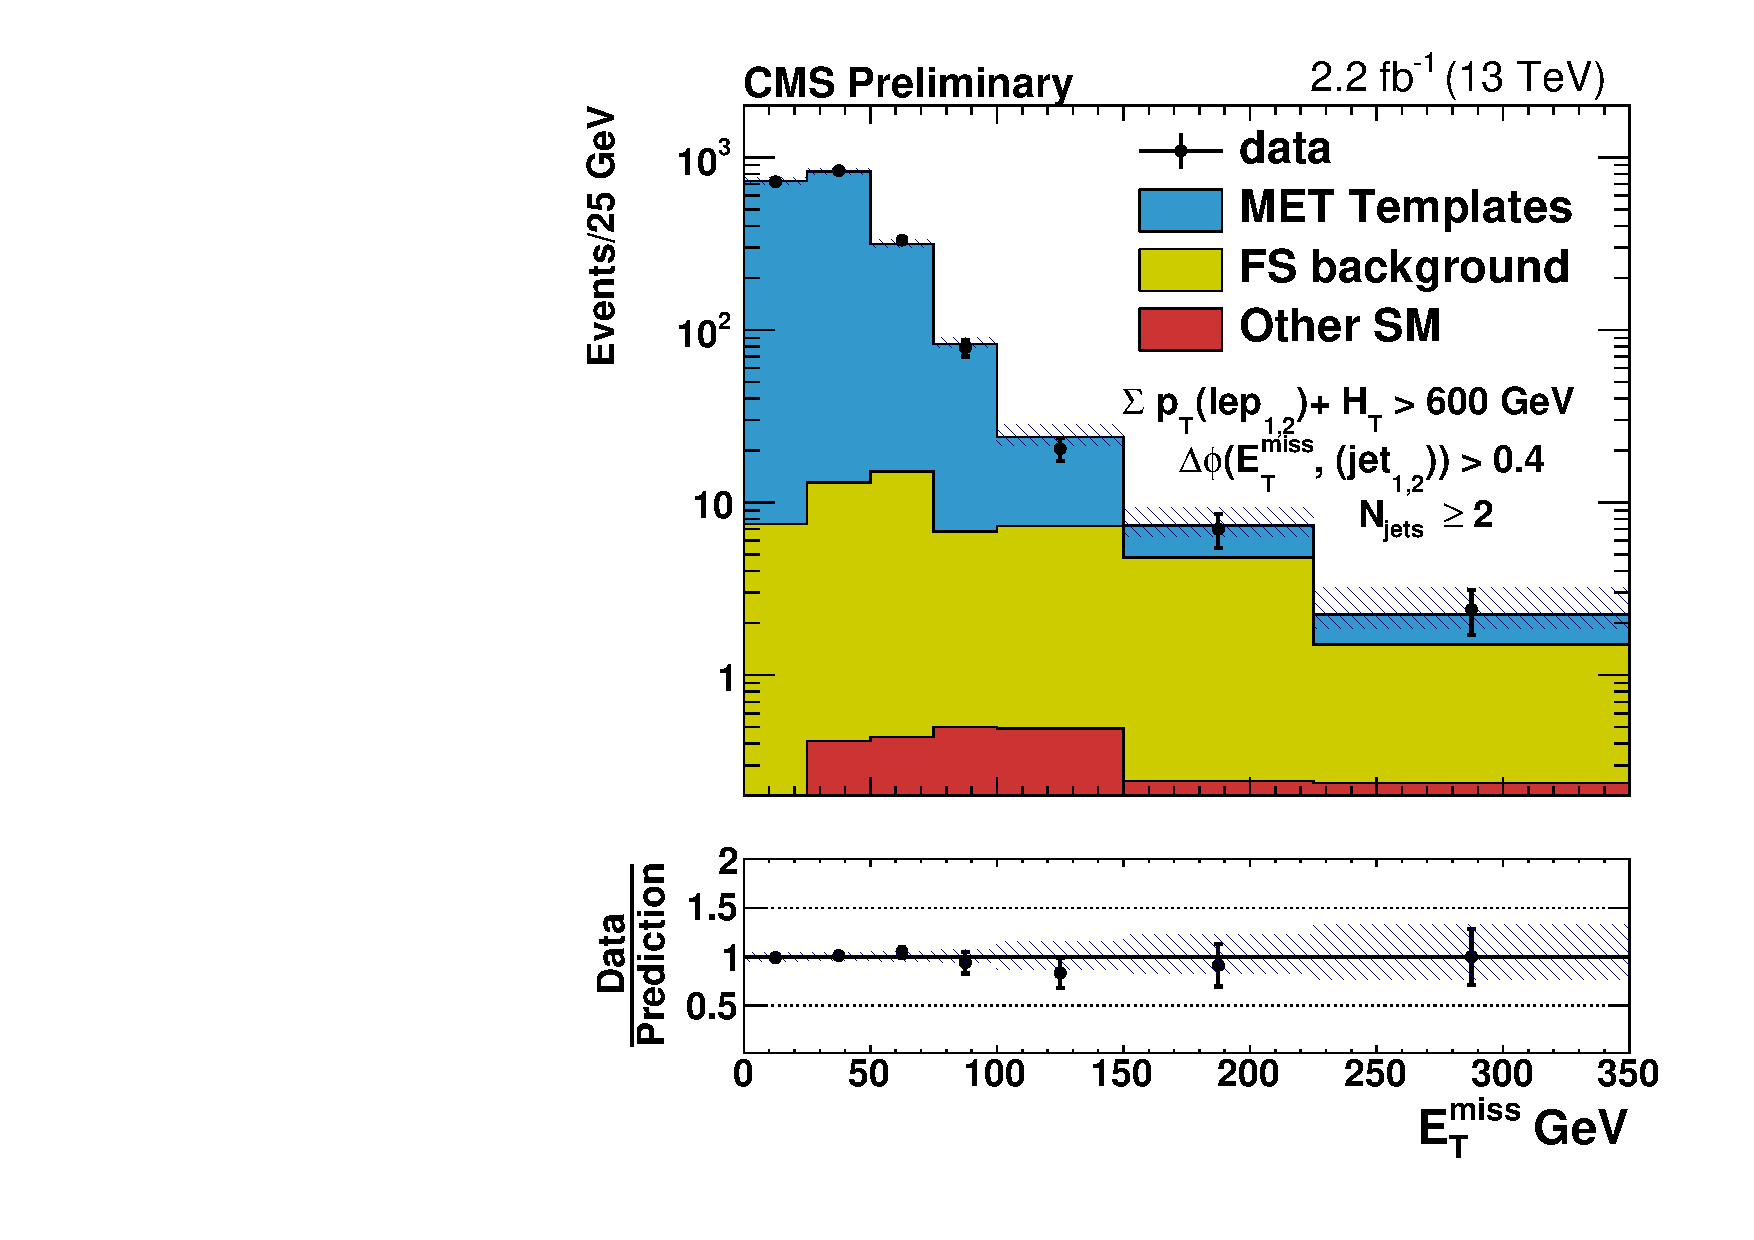
\includegraphics[width=0.8\textwidth]{results/figs/h_met_rawgt1jet_ll_signalregion_rawMET_loosephoton_SR_ATLAS_fsbkg_passtrig.pdf} \\
\end{tabular}
\caption{The \MET\ distribution is shown for data vs. the data-driven predictions in the ATLAS signal region.
See Tables~\ref{tab:results_bveto_SRA}~and~\ref{tab:results_SR_ATLAS}~for yields.
\label{fig:results_SR_ATLAS}
}
\end{center}
\end{figure}

\subsection{Interpretations}


In this analysis, we interpret the results of this search in the T5ZZ model.
The model is expected to have many jets, so most of the sensitivity comes from SRB.
We observe an expected and observed upper limit for gluinos with mass up to 1.3 TeV when the neutralino mass is large,
and when the neutralino mass is small the expected (observed) upper limit is around 1.2 (1.1) TeV.
These results show a significant improvement over the 8 TeV result where we saw an observed and expected limit for gluino masses from 1 to 1.1 TeV.


\begin{figure}[!htb]
\begin{center}
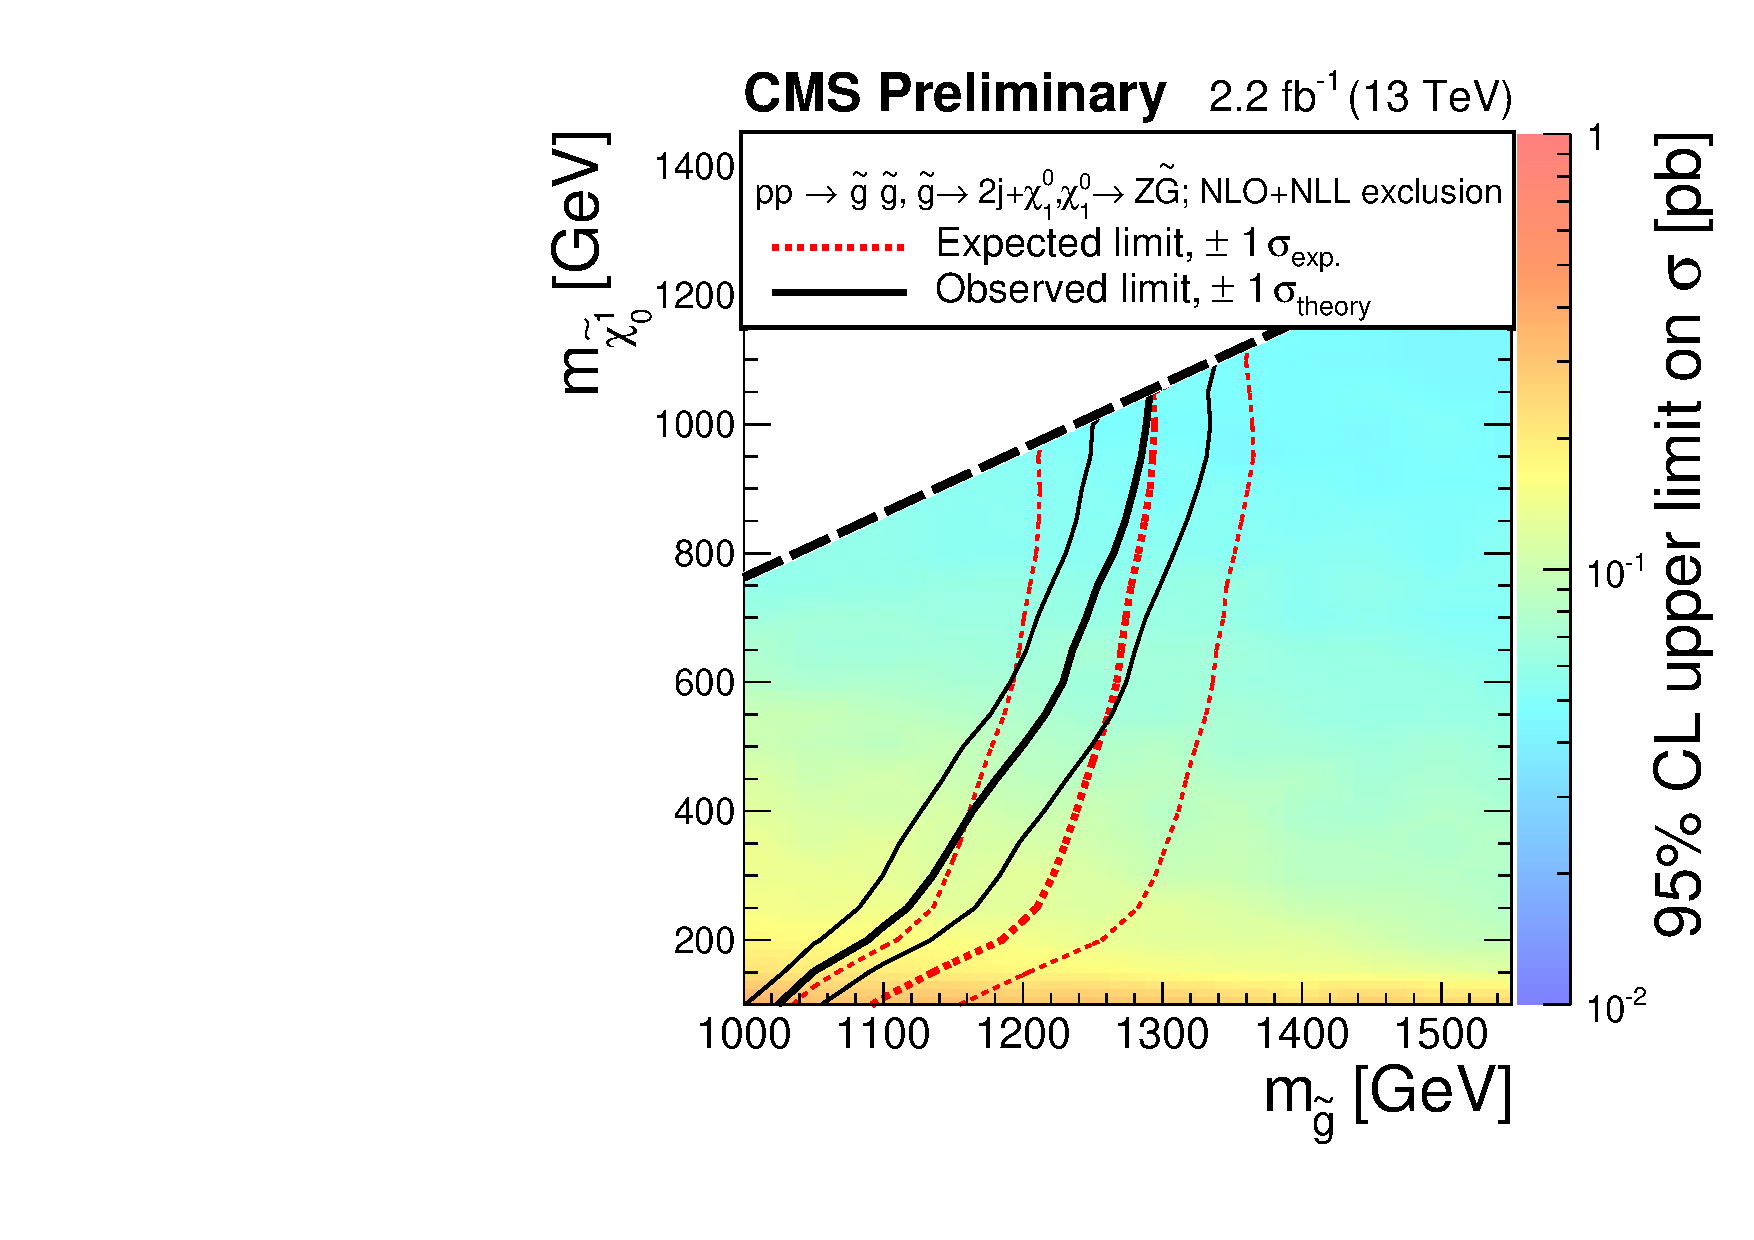
\includegraphics[width=0.8\textwidth]{results/figs/T5ZZ_Exclusion_13TeV.pdf}
\caption{ Exclusion contours are shown when we interpret the results of this analysis in the T5ZZ model.
  Everything to the left of the red (black) dotted line shows the masses which are exlcuded by the expected (observed) limit.
\label{fig:results_T5ZZ}}
\end{center}
\end{figure}


\clearpage
